% Interim submission report — TRP1 Week 5: Agentic Event Store & Enterprise Audit Infrastructure
% Compile: pdflatex INTERIM_SUBMISSION_REPORT.tex (run twice if references used)

\documentclass[11pt,a4paper]{article}
\usepackage[utf8]{inputenc}
\usepackage[T1]{fontenc}
\usepackage{lmodern}
\usepackage{geometry}
\usepackage{hyperref}
\usepackage{graphicx}
\usepackage{booktabs}
\usepackage{enumitem}
\usepackage{tikz}
\usetikzlibrary{arrows.meta,positioning,shapes.geometric}

\geometry{margin=2.5cm}
\hypersetup{colorlinks=true,linkcolor=blue,urlcolor=blue,citecolor=blue}

\title{\textbf{Interim Submission Report}\\[0.5em]
\large The Ledger: Agentic Event Store \& Enterprise Audit Infrastructure}
\author{TRP1 Week 5}
\date{\today}

\begin{document}
\maketitle
\tableofcontents
\newpage

% ---------------------------------------------------------------------------
\section{Conceptual Foundations: EDA vs.\ Event Sourcing and Aggregate Boundaries}

\subsection{EDA vs.\ Event Sourcing (precise distinction)}

\textbf{Event-Driven Architecture (EDA)} describes systems where components communicate by emitting \emph{messages} or \emph{notifications}. In practice, many ``agent traces'' are implemented with callbacks (e.g.\ LangChain-style tracing): the trace is a \emph{side channel}. Such data can be \textbf{dropped}, \textbf{buffer-limited}, or \textbf{never durably committed} as the system's source of truth. EDA is appropriate for telemetry and integration, but it does not guarantee an auditable, replayable record of business facts.

\textbf{Event Sourcing (ES)} treats the append-only event log as the \textbf{authoritative record of state}. Events are facts; they are persisted before (or as part of) the authoritative state transition. They \textbf{cannot be silently discarded} if the operation is accepted: the write path commits them to durable storage (here, PostgreSQL) under ACID semantics.

\textbf{Redesign with The Ledger: what changes and what is gained}
\begin{itemize}[leftmargin=*]
  \item \textbf{What changes:} Callback-based tracing becomes a \emph{secondary} concern. Primary facts (credit analysis completed, compliance rule outcomes, human review, orchestrator decision) are recorded as \textbf{typed domain events} on named streams. Downstream systems stop inferring history from logs and instead \textbf{replay or project} from the store.
  \item \textbf{What is gained (minimum):}
    \begin{itemize}
      \item \textbf{Replayability:} Any decision can be reconstructed by replaying its aggregate's stream (or relevant global order).
      \item \textbf{Temporal compliance:} Compliance and audit read models can answer ``what did we believe at time $t$?'' by replaying or querying projection snapshots as-of a timestamp (design target; full temporal UI is final-scope).
      \item \textbf{Governance:} Evidence binds to hashes and rule versions in the event payload, not to ephemeral process memory.
    \end{itemize}
\end{itemize}

\subsection{Aggregate boundaries: alternative considered and failure mode}

\textbf{Chosen boundaries (excerpt):} \texttt{LoanApplication} (stream \texttt{loan-\{application\_id\}}), \texttt{ComplianceRecord} (stream \texttt{compliance-\{application\_id\}}), \texttt{AgentSession} (stream \texttt{agent-\{agent\_id\}-\{session\_id\}}), \texttt{AuditLedger} (stream \texttt{audit-\{entity\_type\}-\{entity\_id\}}).

\textbf{Alternative boundary considered (and rejected):} merge \textbf{ComplianceRecord} into \textbf{LoanApplication} so that all compliance writes occur on the loan stream.

\textbf{Coupling introduced by merging:} every compliance rule evaluation would require an append to \texttt{loan-\{id\}}. Under concurrent agent activity (multiple agents writing compliance outcomes, fraud signals, and orchestration steps), all writers contend on the \textbf{same optimistic concurrency key}.

\textbf{Specific failure mode:} suppose a \texttt{ComplianceRuleFailed} append and a \texttt{CreditAnalysisCompleted}-related command both target the merged stream. The compliance write would force the loan aggregate's version to advance; a concurrent credit-analysis append with \texttt{expected\_version} from a stale read would fail with \texttt{OptimisticConcurrencyError}. Worse, to enforce ``compliance cannot be written without loan state X'' you would be tempted to hold \textbf{logical locks} across domains or reorder unrelated facts, increasing contention and coupling regulatory writes to unrelated lifecycle transitions. Keeping compliance on \texttt{compliance-\{application\_id\}} isolates those writes and lets the loan aggregate enforce invariants via \textbf{references and checks across streams} (eventual consistency on read) rather than serializing unrelated domains on one stream.

% ---------------------------------------------------------------------------
\section{Operational Mechanics: Concurrency Control and Projection Lag}

\subsection{Concurrency: full sequence (no hand-waving)}

Assume two agents both observe \textbf{stream version 3} for \texttt{loan-\{id\}} and each issues an append of one event with \texttt{expected\_version = 3}.

\begin{enumerate}[leftmargin=*]
  \item \textbf{Both read} the same logical state: current stream version is 3 (from their last load or from a prior decision).
  \item \textbf{Both call} \texttt{append(stream\_id, events, expected\_version=3)}.
  \item The store begins a \textbf{transaction}, locks the \texttt{event\_streams} row for \texttt{stream\_id} (\texttt{FOR UPDATE}), and compares \texttt{current\_version} to \texttt{expected\_version}.
  \item \textbf{First committer:} \texttt{current\_version == 3} matches; events are inserted at positions 4\ldots; \texttt{current\_version} is updated to 4; outbox rows are written in the \textbf{same} transaction; transaction commits.
  \item \textbf{Second committer:} after the first commit, \texttt{current\_version} is 4. The check \texttt{expected\_version == 3} fails. The implementation raises \textbf{\texttt{OptimisticConcurrencyError}} with \texttt{actual\_version = 4}.
  \item \textbf{Losing agent:} must \textbf{reload} the stream (or reload aggregate state), inspect the new event at position 4, and decide whether its proposed write is still valid (retry with \texttt{expected\_version = 4}) or abandon/supersede (business policy).
\end{enumerate}

This matches the interim test intent: exactly one append succeeds; stream length becomes 4; the loser surfaces \texttt{OptimisticConcurrencyError} explicitly (not swallowed).

\subsection{Projection lag: system response and UI contract}

\textbf{Fact:} read models updated by an async daemon are \textbf{eventually consistent}. A typical lag (e.g.\ 200\,ms) means a user may query a projection immediately after a write and see a \textbf{stale} value (e.g.\ old credit limit).

\textbf{System response:}
\begin{itemize}[leftmargin=*]
  \item Expose \textbf{projection lag} per projection: difference between latest \texttt{global\_position} in \texttt{events} and the projection checkpoint (or equivalent), optionally surfaced as milliseconds using \texttt{recorded\_at} deltas.
  \item For \textbf{critical reads} (e.g.\ disbursement confirmation), the API may offer \textbf{read-your-writes} for a correlation: wait until checkpoint $\geq$ the write's global position, or return \texttt{202 Accepted} with a \textbf{poll URL} until the projection catches up.
\end{itemize}

\textbf{UI contract:} show \textbf{``data as of''} timestamp and, if lag $>$ threshold, a non-blocking banner: ``Updating\ldots last confirmed at $t$'' rather than treating sub-500\,ms lag as an error. For regulated fields, the UI may disable the next step until lag $<$ SLO or until a strong-consistency read path is used.

\textbf{Tradeoff framed explicitly:} sub-500\,ms projection lag for \texttt{ApplicationSummary} is an \textbf{accepted SLO}, not proof of inconsistency; the user is informed of freshness, not blocked by normal eventual consistency.

% ---------------------------------------------------------------------------
\section{Advanced Patterns: Upcasting and Distributed Projection Coordination}

\subsection{Upcasting: structurally correct inference}

\textbf{CreditAnalysisCompleted v1 $\rightarrow$ v2} (illustrative policy aligned with the rubric):

\begin{verbatim}
def upcast_credit_v1_to_v2(payload: dict, recorded_at) -> dict:
    return {
        **payload,
        "model_version": infer_model_from_deployment_timeline(recorded_at),  # approximate
        "confidence_score": None,  # unknown at source; do not fabricate
        "regulatory_basis": infer_active_rule_versions_at(recorded_at),
    }
\end{verbatim}

\textbf{Field-level reasoning:}
\begin{itemize}[leftmargin=*]
  \item \textbf{confidence\_score = null:} The historical event never computed a score. \textbf{Fabricating} a numeric score would imply false precision for regulators and would corrupt analytics (downstream treats it as measured). \textbf{Null} means ``absent''; dashboards and compliance workflows must handle unknown explicitly.
  \item \textbf{model\_version (inference):} Derived from \texttt{recorded\_at} against a \textbf{known deployment timeline}; labeled as \textbf{approximate} in metadata or documentation where required.
  \item \textbf{regulatory\_basis:} Inferred from \textbf{rule versions active at \texttt{recorded\_at}}; documented as inference, not primary-source unless cross-checked.
\end{itemize}

\textbf{Unknown vs.\ inferrable:} Genuinely unknown quantities that were never produced must remain \textbf{null}. Quantities derivable from external, versioned policy tables may be \textbf{inferred with documented uncertainty}; the system must not conflate the two.

\subsection{Distributed projection coordination}

\textbf{Primitive:} a single-writer lease implemented with \textbf{PostgreSQL advisory locks} or a \textbf{lease row} (\texttt{SELECT \ldots FOR UPDATE SKIP LOCKED}) in a \texttt{projection\_leader} table, combined with \textbf{checkpointed} consumption of \texttt{events} by \texttt{global\_position}.

\textbf{Failure mode without coordination:} two daemon nodes process the same batch of events and apply the same projection updates twice, \textbf{double-counting} aggregates (e.g.\ \texttt{analyses\_completed}) and corrupting metrics.

\textbf{Recovery when the leader fails:} the lease expires (TTL) or the lock is released on process death; a follower acquires the lock, \textbf{reloads the last committed checkpoint} from \texttt{projection\_checkpoints}, and resumes from the next \texttt{global\_position}. Idempotent projection writes (e.g.\ upserts keyed by \texttt{(application\_id, global\_position)}) reduce duplicate-application harm during handover; the rubric-pure fix is \textbf{exactly one active processor} per projection group at a time.

% ---------------------------------------------------------------------------
\section{Architecture Diagram}

Figure~\ref{fig:arch} shows the central persistence layer, aggregate streams, command path, and outbox as part of the same append transaction.

\begin{figure}[htbp]
\centering
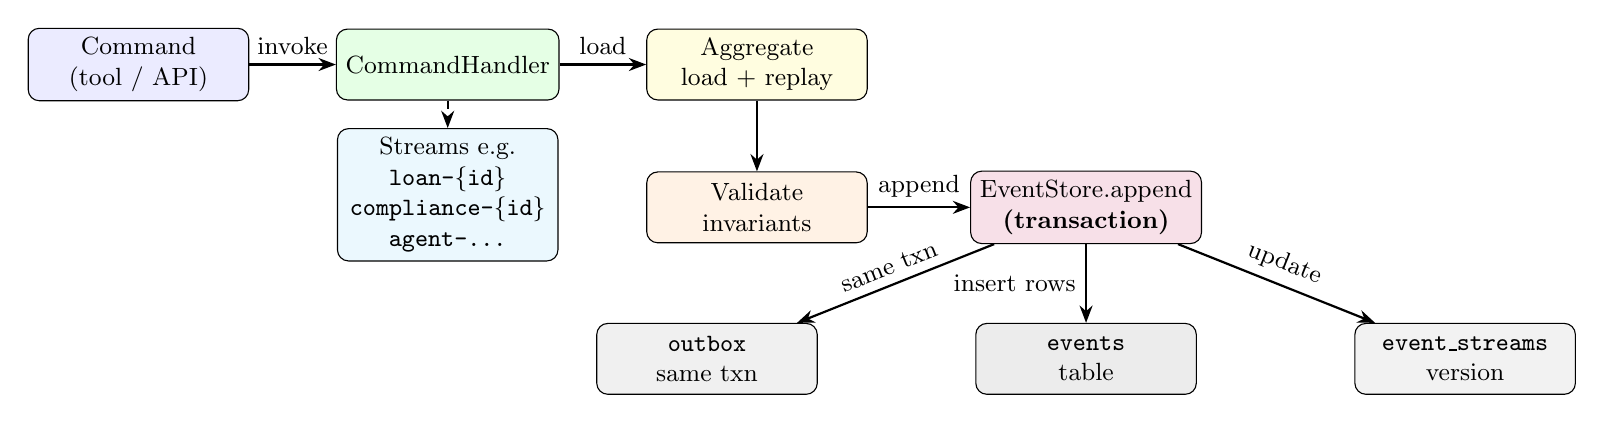
\begin{tikzpicture}[
  font=\small,
  box/.style={draw,rounded corners,minimum width=2.8cm,minimum height=0.9cm,align=center},
  arrow/.style={-{Stealth[length=2.2mm]},thick},
]

\node[box,fill=blue!8] (cmd) {Command\\(tool / API)};
\node[box,right=1.1cm of cmd,fill=green!10] (handler) {CommandHandler};
\node[box,right=1.1cm of handler,fill=yellow!12] (agg) {Aggregate\\load + replay};
\node[box,below=0.9cm of agg,fill=orange!10] (val) {Validate\\invariants};
\node[box,right=1.3cm of val,fill=purple!12] (es) {EventStore.append\\\textbf{(transaction)}};

\node[box,below=1.0cm of es,fill=gray!15] (ev) {\texttt{events}\\table};
\node[box,left=2.0cm of ev,fill=gray!12] (out) {\texttt{outbox}\\same txn};
\node[box,right=2.0cm of ev,fill=gray!10] (str) {\texttt{event\_streams}\\version};

\node[box,below=0.35cm of handler,fill=cyan!8] (streams) {Streams e.g.\\\texttt{loan-\{id\}}\\\texttt{compliance-\{id\}}\\\texttt{agent-\ldots}};

\draw[arrow] (cmd) -- node[above,sloped] {invoke} (handler);
\draw[arrow] (handler) -- node[above,sloped] {load} (agg);
\draw[arrow] (agg) -- (val);
\draw[arrow] (val) -- node[above] {append} (es);
\draw[arrow] (es) -- node[left] {insert rows} (ev);
\draw[arrow] (es) -- node[above,sloped] {same txn} (out);
\draw[arrow] (es) -- node[above,sloped] {update} (str);
\draw[arrow,dashed] (handler.south) -- (streams.north);

\end{tikzpicture}
\caption{Command path: Command $\rightarrow$ CommandHandler $\rightarrow$ Aggregate (replay) $\rightarrow$ validation $\rightarrow$ append. Outbox is written in the \textbf{same} transaction as \texttt{events}, not as a separate step.}
\label{fig:arch}
\end{figure}

\noindent\textbf{Trace one event (reader-only):} Command $\rightarrow$ Handler loads aggregate from stream $\rightarrow$ validation $\rightarrow$ \texttt{EventStore.append} $\rightarrow$ rows in \texttt{events} + \texttt{outbox} + \texttt{event\_streams} updated atomically.

% ---------------------------------------------------------------------------
\section{Progress Evidence and Gap Analysis}

\subsection{Working (interim)}

\begin{itemize}[leftmargin=*]
  \item PostgreSQL schema: \texttt{events}, \texttt{event\_streams}, \texttt{projection\_checkpoints}, \texttt{outbox}; projection tables for read models.
  \item \textbf{EventStore:} append with \texttt{expected\_version}, load with upcasting hook, outbox in same transaction.
  \item \textbf{Aggregates / handlers:} loan and agent session with explicit transition checks; \texttt{expected\_version} derived from \texttt{expected\_version\_for\_append()} on loaded aggregates.
  \item \textbf{Tests:} double-decision concurrency; upcasting immutability; Gas Town recovery sketch; MCP-style lifecycle smoke test.
\end{itemize}

\subsection{Test evidence (concurrency — assertions required by rubric)}

When PostgreSQL is running and \texttt{DATABASE_URL} is set, \texttt{pytest} for the concurrency test checks:
\begin{itemize}[leftmargin=*]
  \item Total events on the stream after concurrent appends = \textbf{4} (not 5).
  \item Winning append results in last event \texttt{stream\_position = 4}.
  \item Losing task receives \textbf{\texttt{OptimisticConcurrencyError}} (via \texttt{asyncio.gather(..., return\_exceptions=True)}), not a silent failure.
\end{itemize}

\noindent\textit{Attach: terminal screenshot or log of \texttt{uv run pytest tests/test\_concurrency.py -v} for the PDF.}

\subsection{In progress / gaps (named components + reasons)}

\begin{itemize}[leftmargin=*]
  \item \textbf{Full loan state machine in all handlers:} not every transition in the rubric (e.g.\ compliance $\rightarrow$ decision $\rightarrow$ human $\rightarrow$ final) is wired end-to-end in command handlers; some states are enforced on replay but not exercised by a full MCP-only lifecycle through \texttt{FinalApproved}.
  \item \textbf{Projection daemon fault tolerance:} batch processing exists; \textbf{per-event skip after retry} and idempotent projection keys need hardening for production. A known risk: if checkpoint advances \textbf{before} a projection side-effect is durably applied, crash could \textbf{skip} work; if checkpoint lags after apply, crash could \textbf{reprocess}---mitigated by idempotent upserts where implemented.
  \item \textbf{Compliance temporal snapshots:} \texttt{as\_of} queries are supported at the read-model layer in principle; full snapshot invalidation strategy and SLO demonstration under load are final-scope.
  \item \textbf{MCP tool surface:} interim exposes a subset of tools/resources; all eight tools and six resources with full precondition text and rate limits are stretch goals for final.
\end{itemize}

\subsection{Final submission plan (sequenced, dependency-aware)}

\begin{enumerate}[leftmargin=*]
  \item \textbf{Complete command handlers} for remaining lifecycle events (fraud, compliance, decision, human review) \emph{after} aggregate invariants are stable---depends on loan + compliance aggregate rules.
  \item \textbf{Harden daemon:} transactional checkpointing strategy (checkpoint + projection write ordering), retry policy, and lag metrics under load---depends on stable projection SQL.
  \item \textbf{Expand MCP} to full tool/resource matrix; integration test drives \emph{only} MCP---depends on (1).
  \item \textbf{Bonus:} what-if and regulatory package---depends on trustworthy projections and integrity chain.
\end{enumerate}

\subsection{What I do not yet fully understand (explicit)}

\begin{itemize}[leftmargin=*]
  \item Exact \textbf{idempotency key} strategy for every projection row under at-least-once delivery from the outbox to an external bus (Week~10 bridge).
  \item Whether \textbf{read-your-writes} for a given \texttt{correlation\_id} should block on projection checkpoint or use inline read model updates for a subset of commands.
\end{itemize}

\vspace{1em}
\noindent\rule{\textwidth}{0.4pt}\\
\textit{End of interim report. Compile this file to PDF for submission; embed or attach architecture diagram export if required separately.}

\end{document}
